








\section{Περιγραφή λογισμικού}


Το λογισμικό αυτό αποτελείται από 3 μέρη τα οποία ουσιαστικά αποτελούν και
τις περιφερειακές συσκευές τις οποίες υποστηρίζει για την επίλυση του προβλήματος.
Αυτά είναι το ποντίκι, το πληκτρολόγιο και το χειριστήριο κονσόλας βιντεοπαιχνιδιών.
Προτού όμως ξεκινήσει η αποκλειστική χρήση του συστήματος με μόνο μία από αυτές
τις περιφερειακές συσκευές θα χρειαστεί να γίνει η αρχικοποίηση της εφαρμογής κατά
την πρώτη εκτέλεση του προγράμματος από τον χρήστη. Το πρόγραμμα θα καθοδηγήσει τον
χρήστη θέτοντας μέσω των γραφικών στοιχείων κάποιες απαραίτητες για την εκτέλεση
τις εφαρμογής παραμέτρους. Οι παράμετροι αυτοί είναι το όνομα του προφίλ του χρήστη
που θα το χρησιμοποιήσει και ένα αρχικό directory στο οποίο βρίσκονται οι περισσότερες
εφαρμογές που είναι εγκατεστημένες στον υπολογιστή. Με αυτόν τον τρόπο η εφαρμογή 
θέτει τις προεπιλεγμένες ρυθμίσεις για το προφίλ του χρήστη και φτάνει στο τελικό
στάδιο που είναι και βασικός στόχος της, δηλαδή η εκτέλεση εφαρμογών.

\section{Εκτέλεση εφαρμογών με το ποντίκι}


Το ποντίκι όπως είναι γνωστό είναι ένα εξαιρετικά απλό μέσο με το οποίο επικοινωνεί
ο χρήστης με τον υπολογιστή και επιτρέπει την χρήση ενός μόνο χεριού για την περιήγηση
μέσα σε αυτόν. Επομένως, η υποστήριξη της συσκευής αυτής από την εφαρμογή γίνεται
μέσω της γραφικής διεπαφής από όπου και είναι εύκολα προσβάσιμα τα στοιχεία που
διαχειρίζονται την εκτέλεση, προσαρμογή και διαχείριση των προγραμμάτων που είναι
εγκατεστημένα στο περιβάλλον του χρήστη. Για τον σκοπό αυτό έχουν προστεθεί τα κατάλληλα
στοιχεία γραφικής διεπαφής που υλοποιούν την προβλεπόμενη από τον τελικό χρήστη 
λειτουργικότητα της εφαρμογής. Πιο συγκεκριμένα, η γραφική διεπαφή έχει χωριστεί σε τρία κομμάτια.
Αυτά υλοποιούνται μέσω του Qt σε καρτέλες οι οποίες στην συνέχεια προστίθενται στο
κεντρικό QTabWidget που αποτελεί κομμάτι τoυ βασικού γραφικού στρώματος του προγράμματος.
Για τις ανάγκες της εφαρμογής έχει δημιουργηθεί μια καρτέλα με τις εφαρμογές που γνωρίζει
η εφαρμογή, μια καρτέλα με τις αγαπημένες εφαρμογές του χρήστη και μια καρτέλα με τις
ρυθμίσεις που μπορεί να αλλάξει ο χρήστης για να φέρει την λειτουργικότητα του προγράμματος
πιο κοντά με τις προσωπικές του προτιμήσεις.

\begin{lstlisting}[language=C++, style=cppstyle]
tabs->addTab(tab_all_apps, "Applications");
tabs->addTab(tab_favorites, "Favorites");
tabs->addTab(tab_settings, "Settings");

layout_root->addWidget(tabs);
\end{lstlisting}

Ας αναλύσουμε τώρα την κάθε καρτέλα ξεχωριστά ξεκινώντας από την καρτέλα των ρυθμίσεων για
λόγους συνοχής.



\subsection{Καρτέλα ρυθμίσεων}

Στην καρτέλα με τις ρυθμίσεις βρίσκονται όλες οι λειτουργίες οι οποίες προσαρμόζουν το
πρόγραμμα στις ανάγκες του χρήστη και λειτουργίες που του επιτρέπουν να διαχειριστεί το
προφίλ του. Επιπλέον, μέσα από αυτήν την καρτέλα ο χρήστης αποκτά πρόσβαση στον εικονικό
πληκτρολόγιο μέσω ενός κουμπιού το οποίο αφορά την περιήγηση μέσω ποντικιού (το εικονικό
πληκτρολόγιο είναι επίσης προσβάσιμο από το χειριστήριο κονσολών βιντεοπαιχνιδιών αλλά η
πρόσβαση σε αυτό γίνεται με διαφορετικό τρόπο). Στην συνέχεια υπάρχουν ρυθμίσεις που αφορούν
τις λίστες με τις εφαρμογές του χρήστη που εμφανίζονται στις καρτέλες Applications και 
Favorites. Υπάρχει το checkbox "Include File Extension" το οποίο συμπεριλαμβάνει την κατάληξη
του αρχείου της εφαρμογής στο όνομα που εμφανίζεται στην λίστα. Στην συνέχεια υπάρχουν
checkboxes που επηρεάζουν τον τρόπο εμφάνισης των λιστών. Αυτά είναι τα "Icon Mode" και
"Wrapping" που καθορίζουν αν η λίστες θα εμφανίζονται σε εικονίδια ή όχι και αντίστοιχα αν τα στοιχεία
της κάθε λίστας εμφανίζονται δίπλα στα υπόλοιπα όταν δεν υπάρχει πλέον χώρος στην ορατή περιοχή.
Στην συνέχεια υπάρχει ένα combo box μέσα από το οποίο ο χρήστης μπορεί να επιλέξει την
θεματολογία που επιθυμεί ανάλογα με τις προτιμήσεις χρωμάτων που έχει. Η εφαρμογή παρέχει τις
θεματολογίες "dark", "light", "red", "green", "blue", "yellow", "orange" και "purple" οι οποίες
εφαρμόζουν μια παλέτα χρωμάτων που βασίζεται στο αντίστοιχο χρώμα του ονόματος της. Στην συνέχεια
ο χρήστης βρίσκει διαθέσιμο ένα combo box μέσω του οποίου μπορεί να μεταβεί σε διαφορετικό προφίλ.
Είναι εφικτή η δημιουργία ενός καινούριου προφίλ από τον χρήστη μετά από την πληκτρολόγηση του
ονόματός του στο input field που υπάρχει στην συνέχεια. Η επιθυμία αφαίρεσης ενός προφίλ μπορεί να
ικανοποιηθεί από την μετάβαση στο εκάστοτε όνομα χρήστη με την επιλογή του κουμπιού
"Delete Current Profile" να ακολουθεί για την ολοκλήρωση της διαδικασίας αυτής. Στο τέλος του πλαισίου
της εφαρμογής υπάρχει μια λίστα με τα directories που έχει προσθέσει χρήστης για την εύρεση εφαρμογών 
από το πρόγραμμα αλλά και εγγραφές με διευθύνσεις μεμονωμένων εφαρμογών στο σύστημα αρχείων.
Μετά την λίστα αυτή υπάρχουν κουμπιά για την προσθήκη η αφαίρεση στοιχείων από την λίστα.

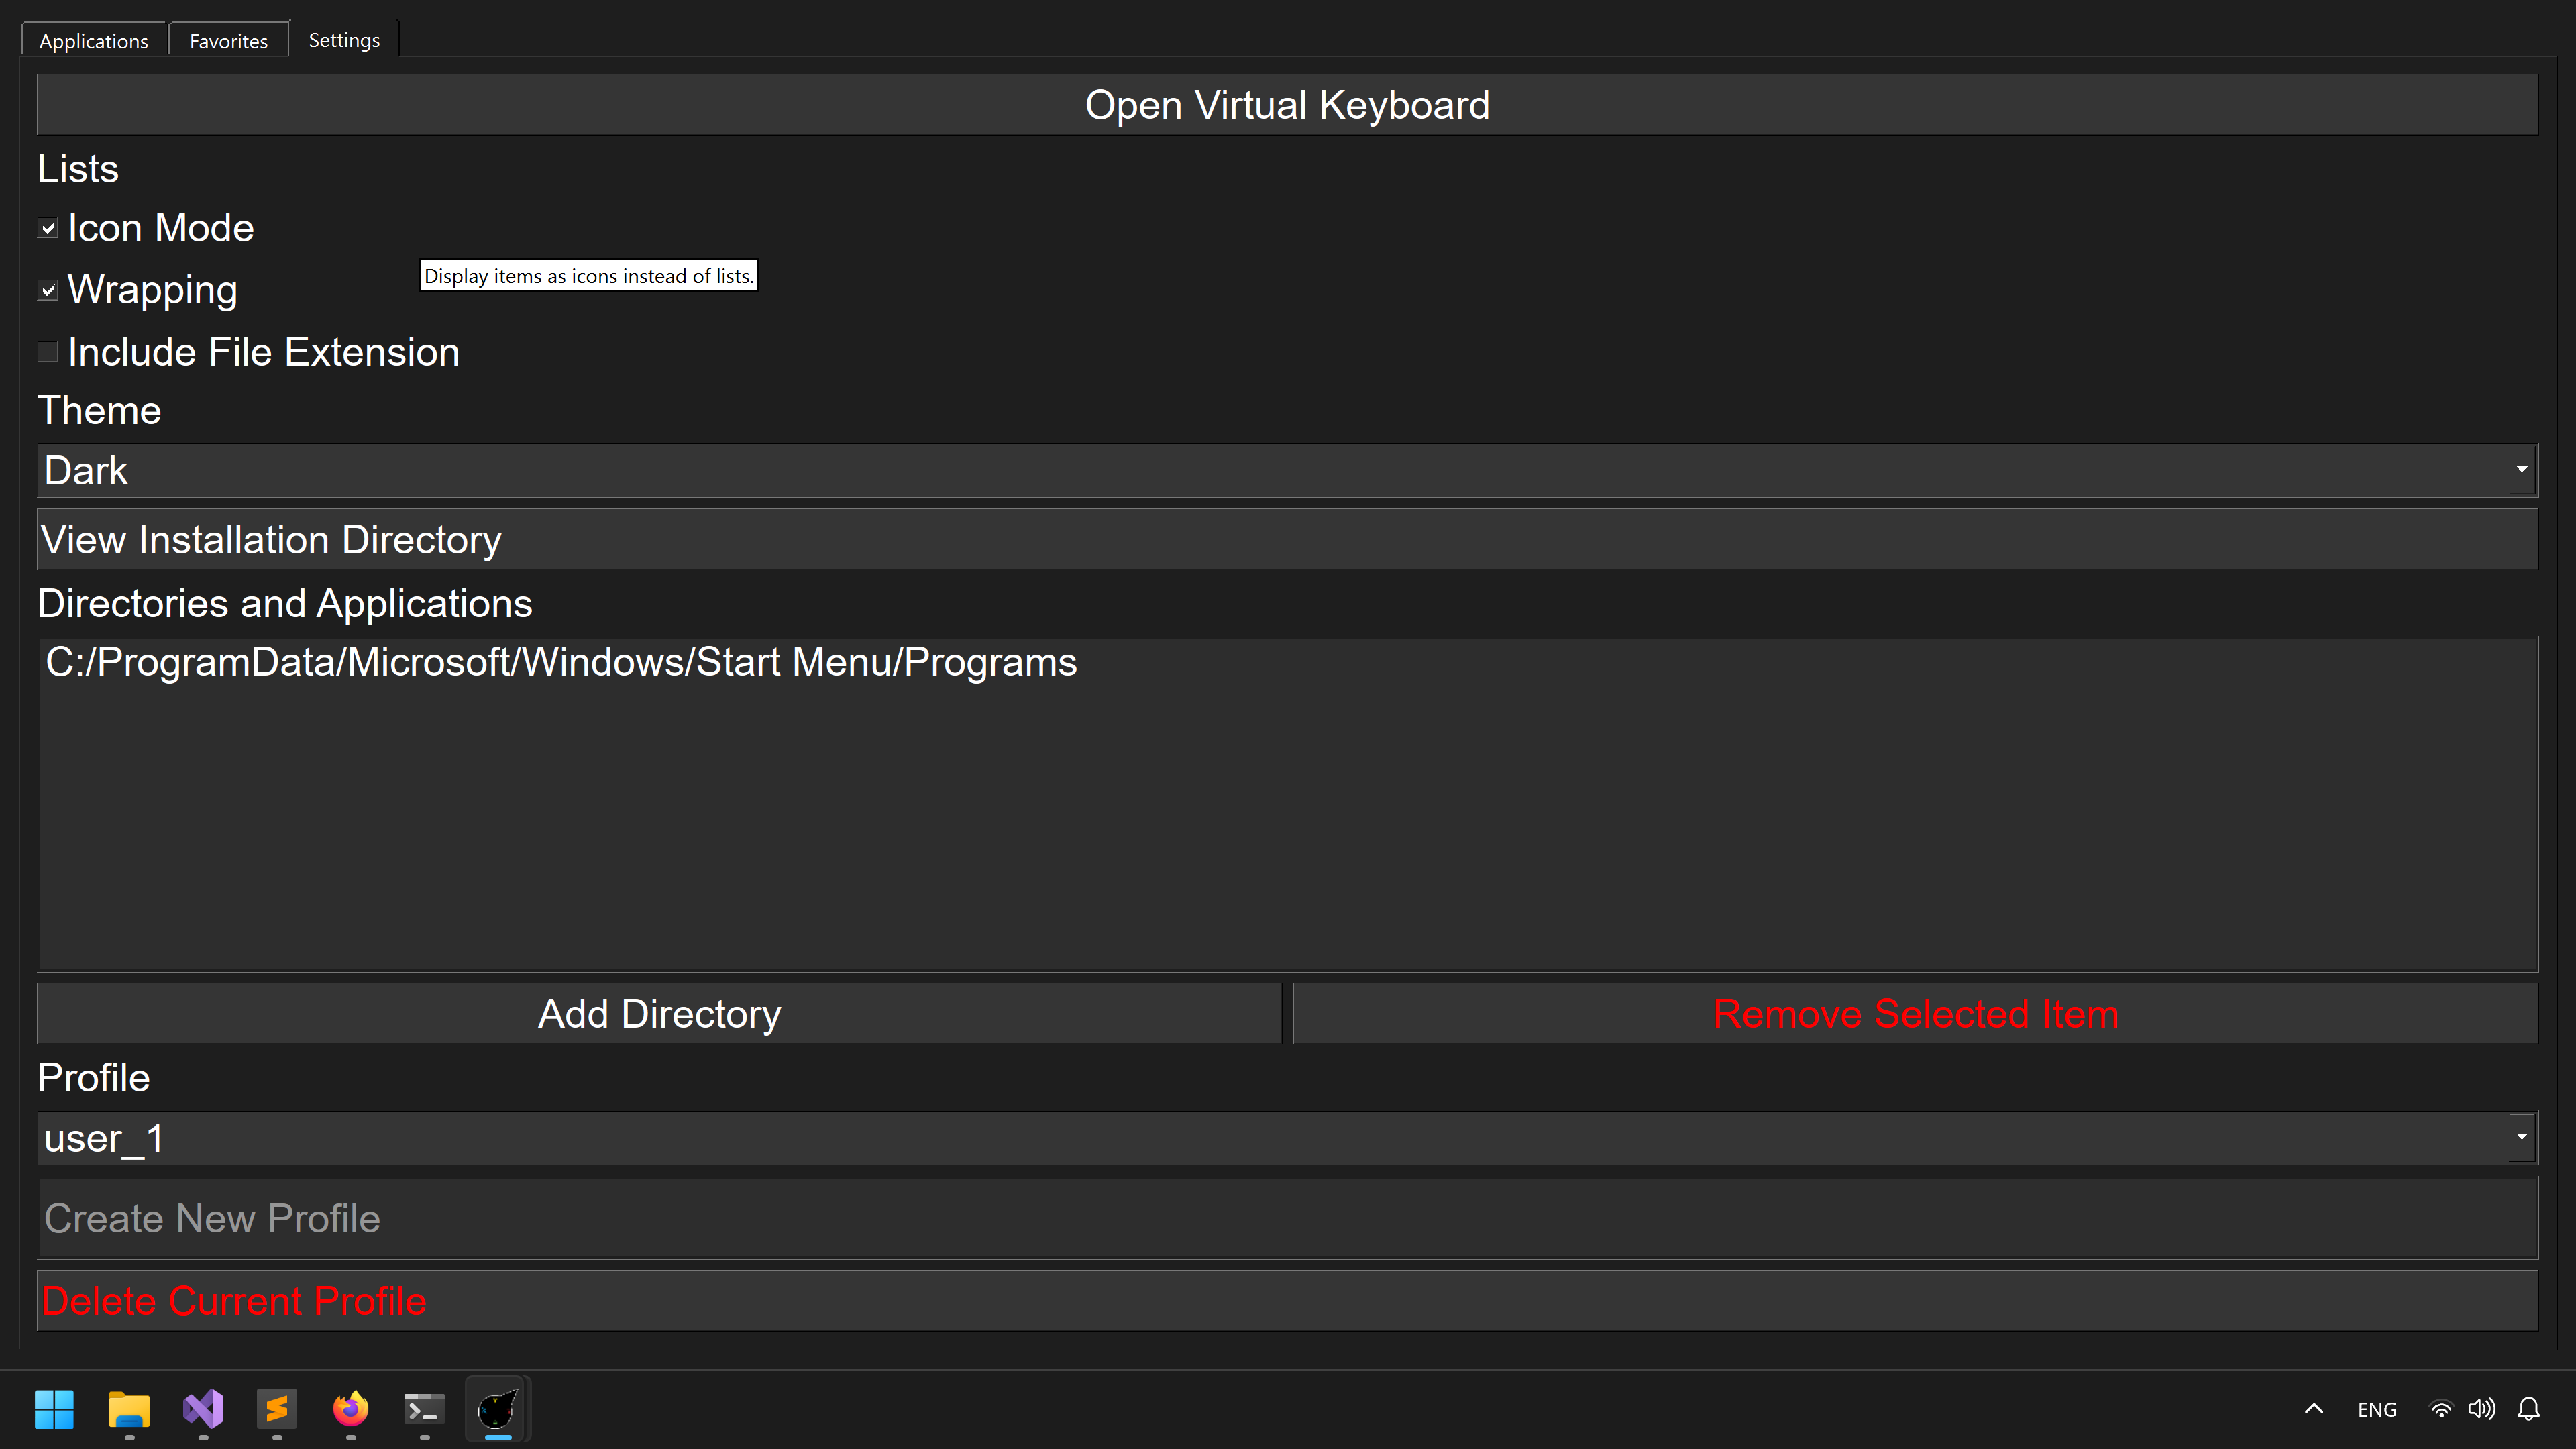
\includegraphics[width=1.0\textwidth]{./images/tab_settings.png}

\subsection{Καρτέλα εφαρμογών}

Έχοντας εξηγήσει την λειτουργία της αρχικοποίησης της εφαρμογής και της προσαρμογής της στις
ανάγκες του χρήστη μέσω της καρτέλας ρυθμίσεων μπορούμε πλέον να προχωρήσουμε στην ανάλυση
της καρτέλας εφαρμογών στην οποία ο ρόλος του προγράμματος πλέον γίνεται εμφανής μέσα από τα
στοιχεία της γραφικής διεπαφής που λύνουν το πρόβλημα που έχει περιγραφεί προηγουμένως. 
Όπως φαίνεται, αρχικά ο χρήστης βλέπει ένα input field. Όπως υποδηλώνεται στο placeholder
κείμενο του input field, σκοπός του στοιχείου αυτού είναι η αναζήτηση εφαρμογών μέσα από την
λίστα εφαρμογών που είναι διαθέσιμη στην εφαρμογή. Με άλλα λόγια, ο χρήστης μπορεί να ψάξει 
ανάμεσα στις εφαρμογές που βλέπει η εφαρμογή μέσω των directories που δόθηκαν και των εφαρμογών
που προστέθηκαν ξεχωριστά. Στην συνέχεια υπάρχει ένα combo box που τροποποιεί την ταξινόμηση
των στοιχείων της λίστας με τις εφαρμογές ανάλογα με την επιλογή του χρήστη σε αύξουσα ή σε
φθίνουσα σειρά. Στην συνέχεια προβάλλονται οι εφαρμογές σε ξεχωριστό πλαίσιο. Ο χρήστης μπορεί
να αξιοποιήσει το ποντίκι για εκτέλεση των εφαρμογών αλλά και για αναζήτηση ανοίγοντας το εικονικό
πληκτρολόγιο μέσα από την καρτέλα ρυθμίσεων. Τέλος, με το δεξί κλικ πάνω στο πλαίσιο εφαρμογών
εμφανίζεται ένα custom context menu μέσα από το οποίο ο χρήστης μπορεί χειροκίνητα να προσθέσει
μεμονωμένες εφαρμογές και να προσθέσει εφαρμογές της λίστας στην λίστα με τα αγαπημένα.

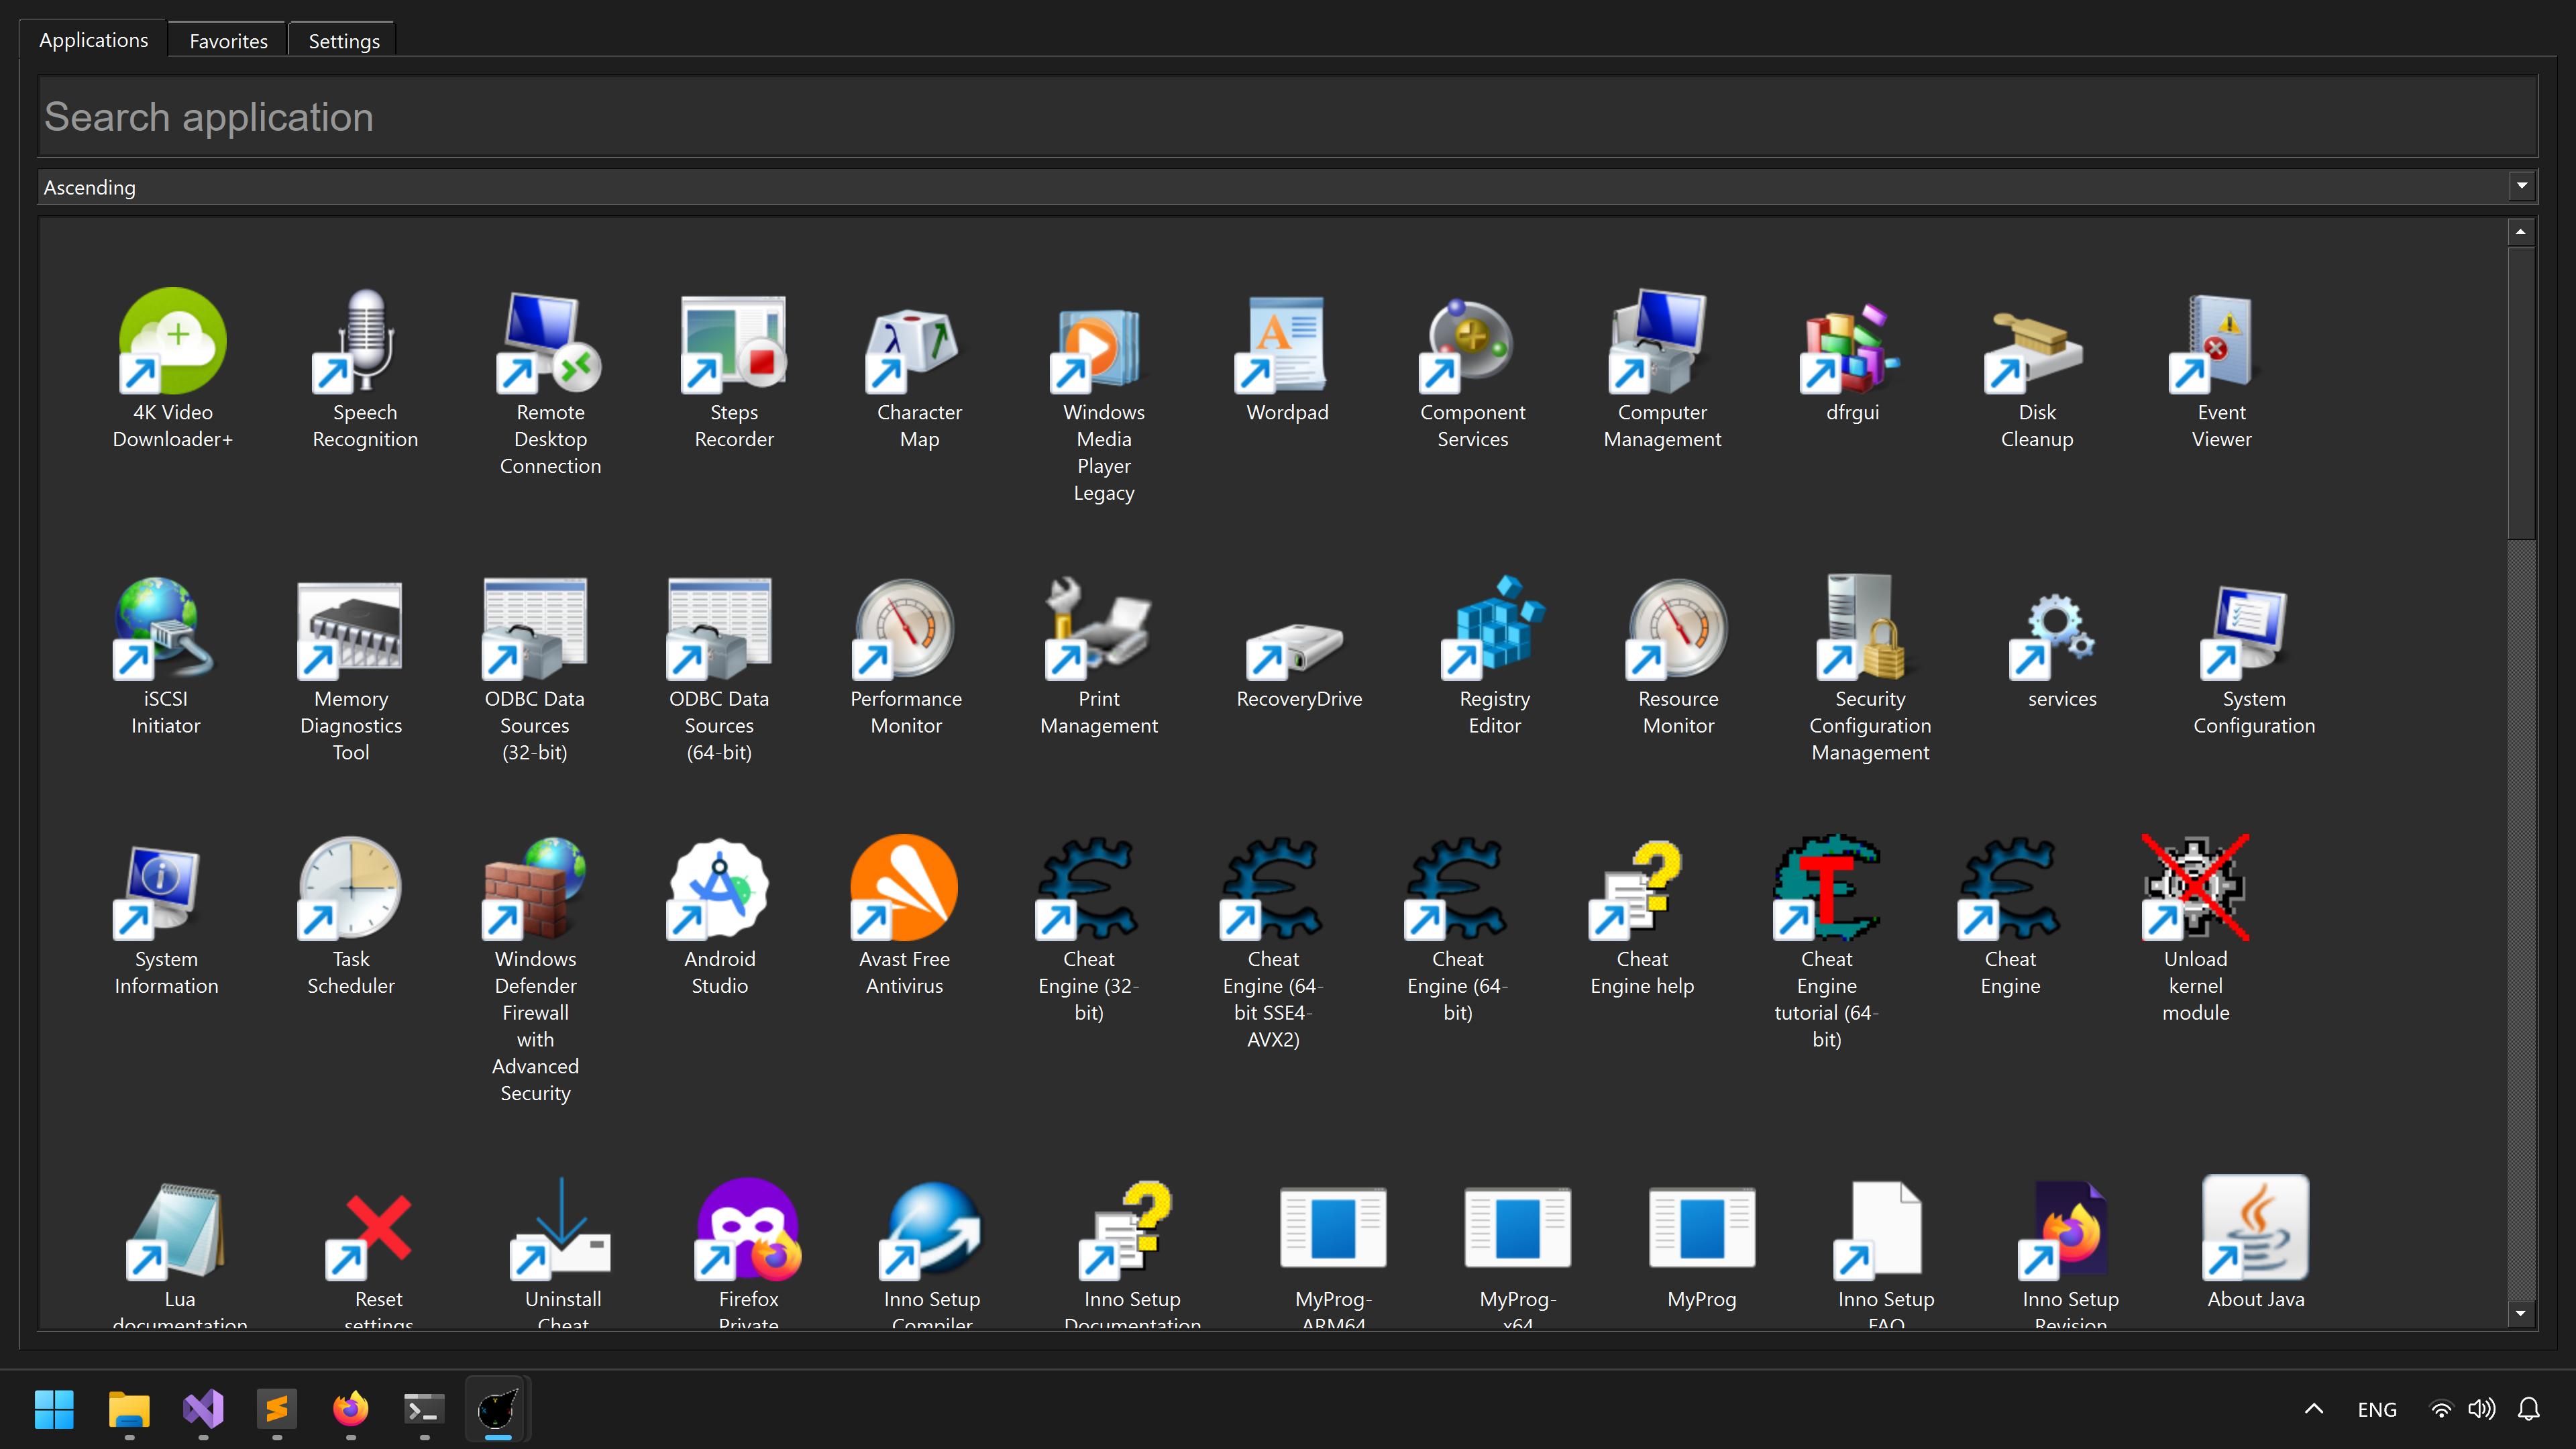
\includegraphics[width=1.0\textwidth]{./images/tab_applications.png}

\subsection{Καρτέλα αγαπημένων εφαρμογών}

Η καρτέλα Favorites δεν έχει κάποια ουσιαστική διαφορά από την βασική καρτέλα εφαρμογών. Στην 
καρτέλα αυτή ο χρήστης θα βρει στοιχεία γραφικής διεπαφής που εμφανίζονται και στην πρώτη καρτέλα
με την μόνη διαφορά να βρίσκεται στην λίστα εφαρμογών που είναι διαφορετική και στο context menu
που πλέον εμφανίζει μόνο επιλογή για αφαίρεση εφαρμογής από την λίστα αγαπημένων.

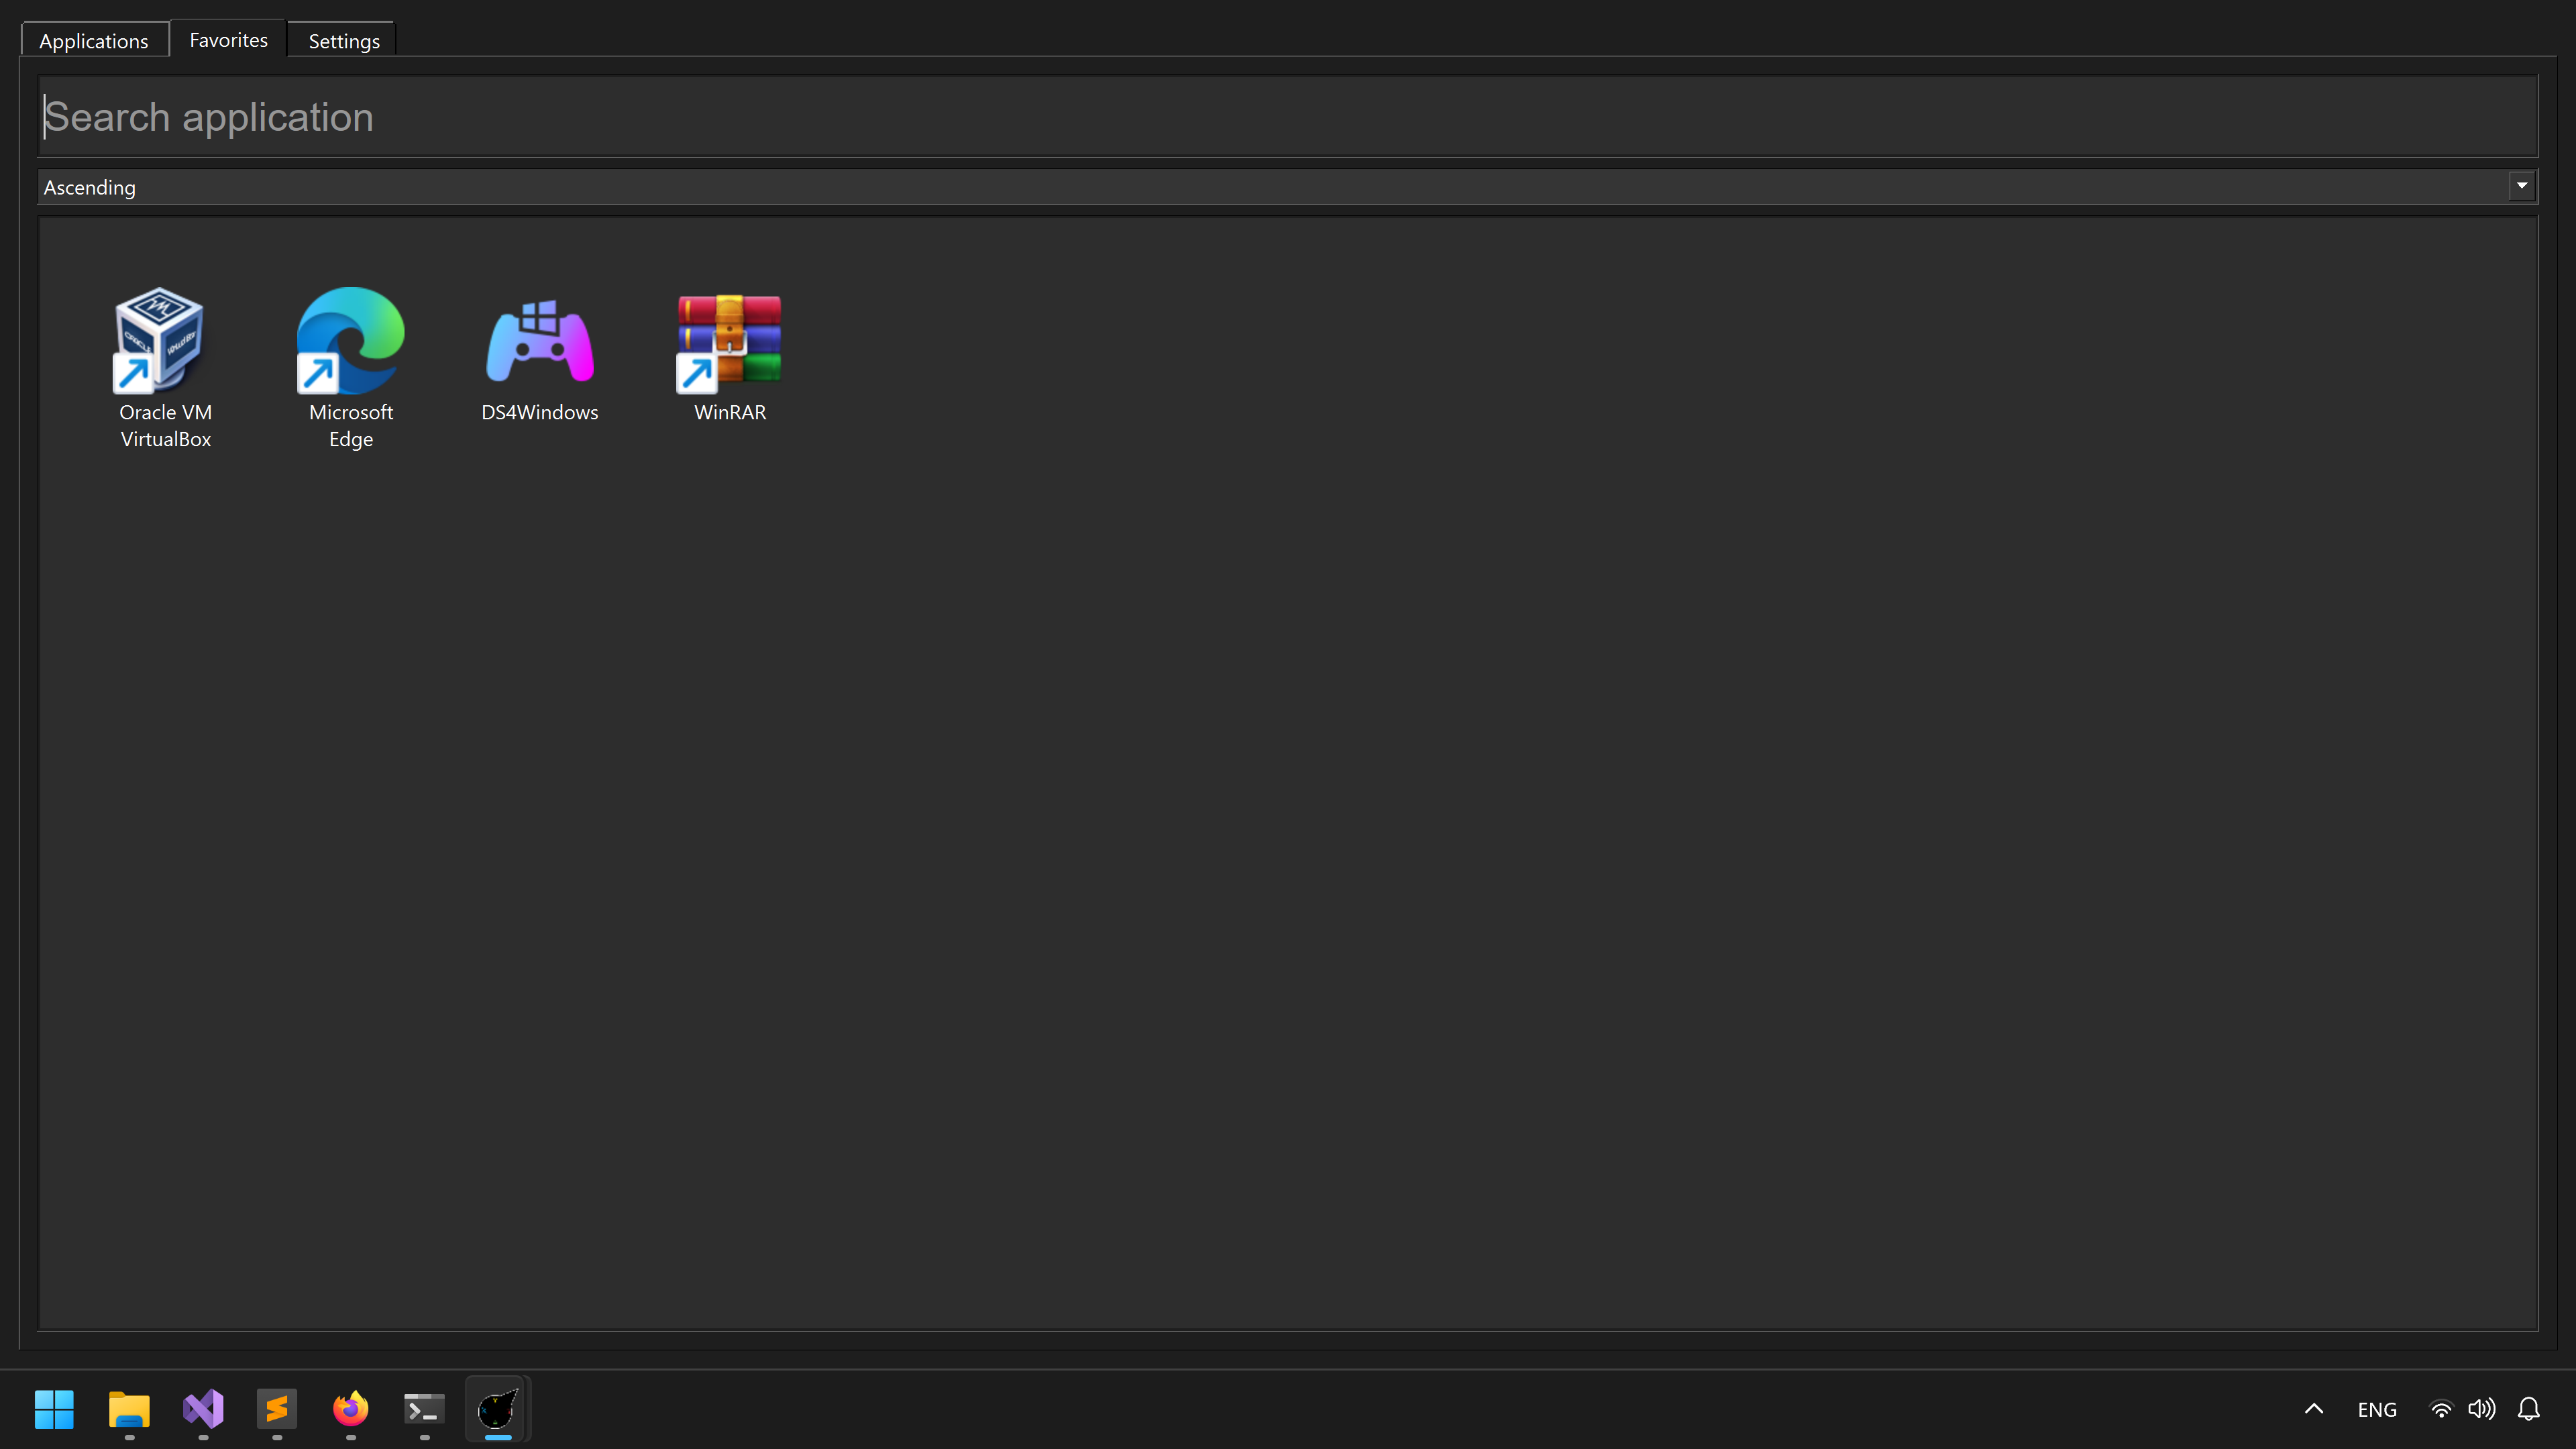
\includegraphics[width=1.0\textwidth]{./images/tab_favorites.png}

\section{Εκτέλεση εφαρμογών με το πληκτρολόγιο}

Σε αντίθεση με το ποντίκι, το πληκτρολόγιο έχει βασική ιδιότητα εισαγωγή κειμένου ως είσοδο στον
υπολογιστή. Επομένως για την εκτέλεση των εφαρμογών μέσω αυτής της συσκευής έχει δημιουργηθεί 
ένα ξεχωριστό παράθυρο μέσα από το οποίο ο χρήστης έχει την δυνατότητα να πληκτρολογήσει για
να αναζητήσει μέσα από την λίστα των προγραμμάτων που γνωρίζει η εφαρμογή. Δηλαδή ή αναζήτηση
γίνεται μέσα στην λίστα εφαρμογών. Με την εισαγωγή κειμένου εμφανίζονται τα αποτελέσματα
αναζήτησης και στην συνέχεια ο χρήστης μπορεί να χρησιμοποιήσει τα βελάκια του πληκτρολογίου
για να μεταβεί στην λίστα με τα αποτελέσματα. Τέλος, πιέζοντας το πλήκτρο Enter εκτελείται η
επιλεγμένη εφαρμογή και το πρόγραμμα κρύβει το παράθυρο εκτέλεσης εφαρμογών. Η επανεμφάνιση του
παραθύρου γίνεται μέσω ενός shortcut που έχει ανατεθεί και γίνεται μέσω του συνδυασμού των πλήκτρων
CTRL + Space. 

\section{Εκτέλεση εφαρμογών με το χειριστήριο βιντεοπαιχνιδιών}

Ένα χειριστήριο βιντεοπαιχνιδιών είναι σχεδιασμένο για τις ανάγκες μιας εμπορικής κονσόλας
βιντεοπαιχνιδιών και συνήθως είναι χρήσιμο στην περιήγηση συστημάτων που είναι σχεδιασμένα
για αυτήν την συσκευή. Όμως ένα λειτουργικό σύστημα όπως το Windows της Microsoft δεν
παρέχει κάποια μητρική υποστήριξη τέτοιου είδους συσκευών. Επομένως χρειάζεται να προστεθεί
λειτουργικότητα από την εφαρμογή για την μετάφραση δεδομένων εισόδου από το χειριστήριο ως
εντολές που επιτρέπουν τον χρήστη να περιηγηθεί στο σύστημα. Για τον σκοπό αυτό αξιοποιούνται
οι διάφορες συντομεύσεις που παρέχει το λειτουργικό σύστημα και υλοποιούνται συναρτήσεις που
επιτρέπουν την εικονική κλήση αυτών των συντομεύσεων αλλά και άλλων εντολών εισόδου του
πληκτρολογίου και του ποντικιού. Επομένως οι εντολές που στέλνονται από το χειριστήριο μεταφράζονται
ως ένας συνδυασμός εντολών πληκτρολογίου και ποντικιού. 